\documentclass[11pt,a4paper]{article}
\usepackage[utf8]{inputenc}
\usepackage[T1]{fontenc}
\usepackage{lmodern}
\usepackage[margin=2.5cm]{geometry}
\usepackage{booktabs}
\usepackage{graphicx}
\usepackage[hidelinks]{hyperref}

\title{An automatic report for the dataset: airline passengers}
\author{Some Math empowered by some AI guided by some researchers}
\date{}

\begin{document}
\maketitle

\noindent\emph{Produced by \texttt{autostat.smc}, a Python port of AutoGP (Saad et al., ICML 2023), with the report writer and model checks of the Automatic Statistician (Lloyd et al., AAAI 2014; Lloyd and Ghahramani, NIPS 2015).}

\begin{center}
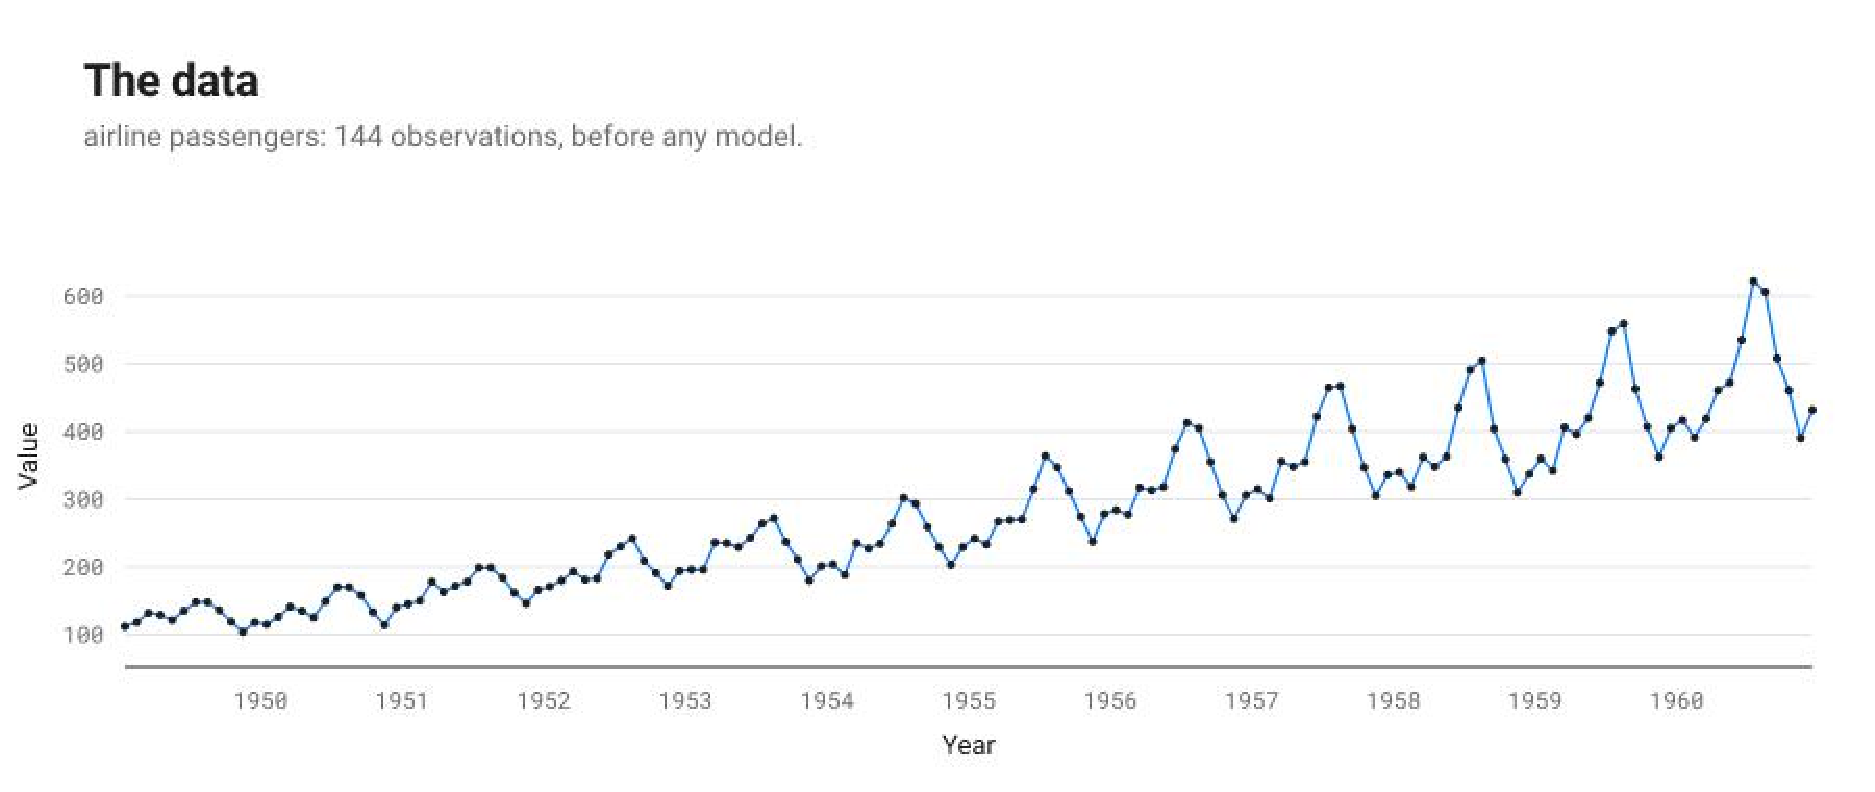
\includegraphics[width=\linewidth]{data.pdf}
\end{center}
\section*{Posterior over structures}

AutoGP keeps no single best structure and runs no BIC search: its stopping point is the end of the data schedule; the weights below replace the comparison of BIC between levels. Each structure's own report gives its formula.

Sequential Monte Carlo kept a weighted population of structures. Forecasts average them by weight. Each structure below is described on its own, with the parameters of its heaviest particle.

\begin{center}
\begin{tabular}{rrll}
\toprule
\# & weight & as 2014 kernels & report \\
\midrule
1 & 0.543 & \texttt{WN + (C + Lin + (C + GE + Lin + Per) x (C + Lin) x (C + Lin) + (C + Lin) x (C + Per)) x (C + Lin)} & \href{structure_1/report.pdf}{\texttt{structure\_1}} \\
2 & 0.276 & \texttt{WN + (C + Lin + Lin + Per + GE x (C + Lin)) x (C + Lin) x (C + Lin)} & \href{structure_2/report.pdf}{\texttt{structure\_2}} \\
3 & 0.089 & \texttt{WN + (C + Lin + Per + GE x (C + Lin) x (C + GE + Lin)) x (C + Lin) x (C + Lin)} & \href{structure_3/report.pdf}{\texttt{structure\_3}} \\
4 & 0.029 & \texttt{WN + (C + Lin) x (C + Lin + Lin + (C + GE + Lin) x (C + Per + GE x (C + Lin) x (C + Lin))) x (C + Lin)} &  \\
5 & 0.028 & \texttt{WN + (C + Lin + Per + (C + Lin) x (C + GE + GE + Lin) x (C + Lin) x (C + Per)) x (C + Lin) x (C + Lin)} &  \\
6 & 0.018 & \texttt{WN + (C + GE + Lin + Per) x (C + Lin) x (C + Lin) x (C + Lin)} &  \\
7 & 0.014 & \texttt{WN + (C + Lin) x (C + GE + Lin + Lin + Per) x (C + Lin) x (C + Lin)} &  \\
8 & 0.002 & \texttt{WN + (C + Lin + Per + (C + Lin) x (C + Lin + Lin) x (C + Lin) x (C + Lin) x (GE + GE)) x (C + Lin) x (C + Lin)} &  \\
\bottomrule
\end{tabular}
\end{center}
\begin{center}
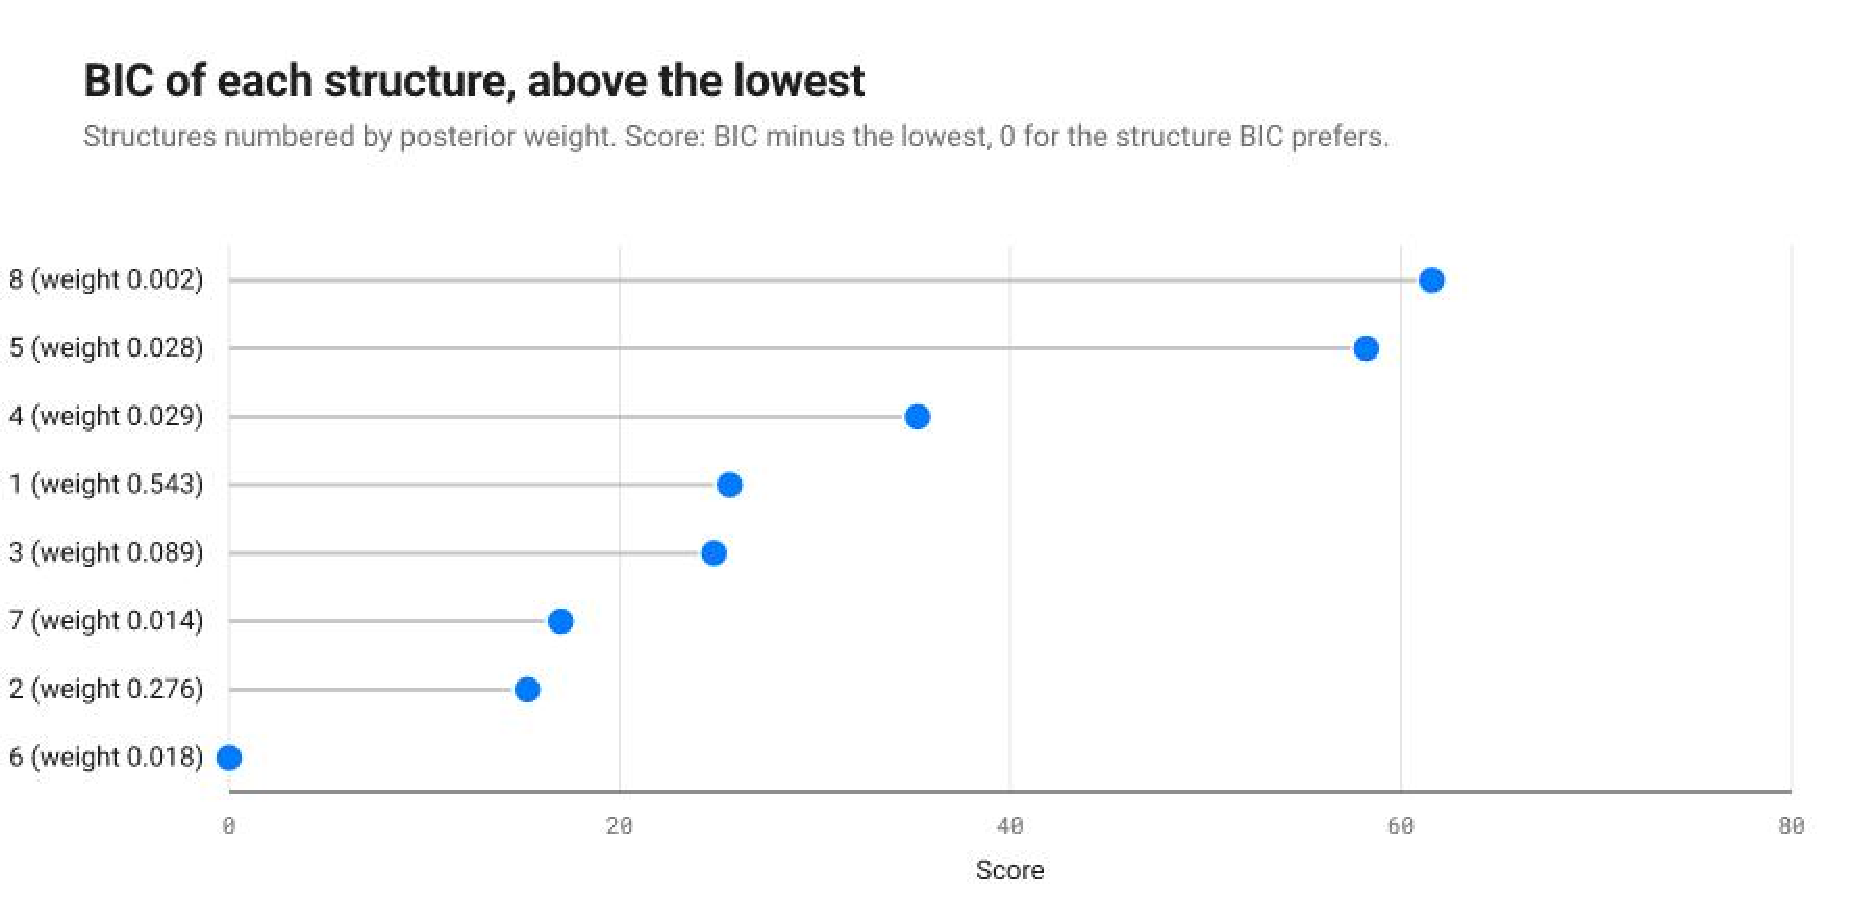
\includegraphics[width=\linewidth]{bic.pdf}
\end{center}

Each structure's BIC is that of its heaviest particle, whose parameters the sampler drew rather than optimised: the BIC the structure could reach is at most this one. BIC and the posterior disagree: BIC ranks structure 6 first (weight 0.018), 25.6 below the heaviest structure.

\section*{Structure 1 (weight 0.543)}

AutoGP formula: \texttt{(Lin * (((Lin * Per) + ((Lin * Lin) * (Lin + (Per + GE)))) + Lin))}.
\begin{enumerate}
  \item A linearly increasing function.
  \item A linearly increasing function.
  \item A quadratic polynomial.
  \item A quadratic polynomial.
  \item A linearly increasing function.
  \item A linearly increasing function.
  \item A quadratic polynomial.
  \item A periodic function with a period of 1.0 years.
  \item A periodic function with a period of 1.0 years but with quadraticly varying amplitude.
  \item A periodic function with a period of 1.0 years but with amplitude increasing linearly away from Aug 1949.
  \item A rough function with marginal standard deviation increasing linearly away from Apr 1950.
  \item A quadratic polynomial.
  \item A linearly increasing function.
  \item A periodic function with a period of 1.0 years but with amplitude increasing linearly away from Mar 1951.
  \item A quadratic polynomial.
  \item A linearly increasing function.
  \item A linearly increasing function.
  \item A quadratic polynomial.
  \item A periodic function with a period of 2.0 years but with amplitude increasing linearly away from Jul 1954.
  \item A rough function.
  \item A rough function with marginal standard deviation increasing linearly away from Mar 1951.
  \item A quadratic polynomial.
  \item A linearly increasing function.
  \item A periodic function with a period of 2.0 years but with amplitude increasing linearly away from Mar 1951.
  \item A periodic function with a period of 2.0 years but with cubicly varying amplitude.
  \item A quadratic polynomial.
  \item Uncorrelated noise.
  \item A periodic function with a period of 2.0 years but with quadraticly varying amplitude.
  \item A periodic function with a period of 2.0 years but with quadraticly varying amplitude.
  \item A rough function with quadraticly varying marginal standard deviation.
  \item A cubic polynomial.
  \item A periodic function with a period of 2.0 years.
  \item A rough function with marginal standard deviation increasing linearly away from Jul 1954.
  \item A periodic function with a period of 2.0 years but with quadraticly varying amplitude.
  \item A quartic polynomial.
  \item A rough function with quadraticly varying marginal standard deviation.
  \item A cubic polynomial.
  \item A periodic function with a period of 2.0 years but with amplitude increasing linearly away from Apr 1950.
  \item A rough function with cubicly varying marginal standard deviation.
  \item A cubic polynomial.
  \item A rough function with quadraticly varying marginal standard deviation.
  \item A cubic polynomial.
  \item A constant.
\end{enumerate}

\section*{Structure 2 (weight 0.276)}

AutoGP formula: \texttt{((Lin * (((Per + (GE * Lin)) + Lin) + Lin)) * Lin)}.
\begin{enumerate}
  \item A linearly increasing function.
  \item A quadratic polynomial.
  \item A linearly increasing function.
  \item A quadratic polynomial.
  \item A linearly increasing function.
  \item A quadratic polynomial.
  \item A rough function with marginal standard deviation increasing linearly away from Dec 1950.
  \item A cubic polynomial.
  \item A quadratic polynomial.
  \item A quadratic polynomial.
  \item A rough function with marginal standard deviation increasing linearly away from Nov 1951.
  \item A periodic function with a period of 1.0 years.
  \item A rough function with quadraticly varying marginal standard deviation.
  \item A periodic function with a period of 1.0 years but with quadraticly varying amplitude.
  \item A periodic function with a period of 1.0 years but with amplitude increasing linearly away from Dec 1950.
  \item A rough function with quadraticly varying marginal standard deviation.
  \item A rough function with marginal standard deviation increasing linearly away from Aug 1953.
  \item A periodic function with a period of 1.0 years but with amplitude increasing linearly away from Nov 1951.
  \item A rough function with quadraticly varying marginal standard deviation.
  \item Uncorrelated noise.
  \item A rough function with cubicly varying marginal standard deviation.
  \item A cubic polynomial.
  \item A rough function.
  \item A linearly increasing function.
  \item A constant.
\end{enumerate}

\section*{Structure 3 (weight 0.089)}

AutoGP formula: \texttt{((Lin * ((Per + (((Lin + GE) * Lin) * GE)) + Lin)) * Lin)}.
\begin{enumerate}
  \item A linearly increasing function.
  \item A linearly increasing function.
  \item A quadratic polynomial.
  \item A quadratic polynomial.
  \item A linearly increasing function.
  \item A quadratic polynomial.
  \item A periodic function with a period of 1.0 years but with amplitude increasing linearly away from Nov 1951.
  \item A periodic function with a period of 1.0 years.
  \item A rough function with marginal standard deviation increasing linearly away from Feb 1950.
  \item A periodic function with a period of 1.0 years but with amplitude increasing linearly away from Jun 1954.
  \item A periodic function with a period of 1.0 years but with quadraticly varying amplitude.
  \item A rough function.
  \item A rough function with quadraticly varying marginal standard deviation.
  \item A rough function with marginal standard deviation increasing linearly away from Nov 1951.
  \item A rough function.
  \item A rough function with marginal standard deviation increasing linearly away from Nov 1951.
  \item A rough function with quadraticly varying marginal standard deviation.
  \item A rough function with marginal standard deviation increasing linearly away from Dec 1951.
  \item A rough function with marginal standard deviation increasing linearly away from Dec 1951.
  \item A rough function with quadraticly varying marginal standard deviation.
  \item A rough function with quadraticly varying marginal standard deviation.
  \item Uncorrelated noise.
  \item A rough function with cubicly varying marginal standard deviation.
  \item A rough function with quadraticly varying marginal standard deviation.
  \item A rough function with cubicly varying marginal standard deviation.
  \item A rough function with quadraticly varying marginal standard deviation.
  \item A rough function with quadraticly varying marginal standard deviation.
  \item A rough function with quarticly varying marginal standard deviation.
  \item A rough function with cubicly varying marginal standard deviation.
  \item A rough function with quadraticly varying marginal standard deviation.
  \item A rough function with cubicly varying marginal standard deviation.
  \item A rough function with marginal standard deviation increasing linearly away from Jun 1954.
  \item A rough function with quadraticly varying marginal standard deviation.
  \item A rough function with cubicly varying marginal standard deviation.
  \item A rough function with marginal standard deviation increasing linearly away from Jun 1954.
  \item A cubic polynomial.
  \item A constant.
\end{enumerate}

\end{document}
